%!TEX root = ../main.tex

\chapter{Methods\label{chap:methods}}
\subsection{Radioactive decay}
Radioactive decay is a process where unstable atomic nucleus transforms into a lower-energy state.
During this process, it loses energy by radiation.
There are three main types of such radiation - alpha, beta and gamma.
Whereas alpha particles can be stopped by a sheet of paper and beta particles by aluminium shielding, gamma particles can be blocked only using a thick block of lead or a massive concrete wall.
Moreover, highly energetic gamma rays have a negative effect on the human body, causing damage on a cellular level.
Being exposed to such radiation poses a risk of severe health problems or death.

\subsection{Some properties of gamma radiation}
The important property of ionizing radiation is that the intensity of the radiation decreases with the inverse square law.
In other words, the intensity at a given point is proportional to $\frac{1}{d^{2}}$, where $d$ is the distance from the source.
The quantity of emitted particles ("strength" of the source) is expressed in Becquerels.
It is a SI unit defined as the number of emitted particles per second.

\subsection{Interaction with matter}
As the gamma particle passes through matter, there are three possible effects that might happen:
\textbf{the photoelectric effect}, \textbf{Compton scattering} and \textbf{pair production}.

\textbf{The photoelectric effect} is typical at low energies of gamma rays. A photon undergoes an interaction with an electron that is bound in an atom. The incident photon completely disappears in this interaction. A product of this interaction is a photon.
\textbf{The Compton effect} is typical for mid-energetic gamma rays. In this process, an incident gamma photon loses energy to an atomic electron. A new lower energetic photon is emitted in a different direction (hence the frequently used term "Compton scattering").
\textbf{Pair production} is typical for high-energetic gamma rays. It is a process in which a photon of sufficient energy is converted into an electron and a positron.

\subsection{Compton effect}
The Compton effect (published in 1923 \cite{}) describes the way how a (gamma or X-ray) photon interacts with a static electron. An incident photon with wavelength $\lambda$ losses some energy to the electron. A new lower energetic photon with wavelength $\lambda^{\prime}$ is emitted under angle $\Theta$. Thanks to the law of conservation of energy and momentum, Compton derived the following equation
\begin{equation}
    \lambda^{\prime} = \lambda + \frac{h}{m_{e}c}(1-\mathrm{cos} \Theta),
\end{equation}
where $\lambda$ is the wavelength of the incident photon, $\lambda^{\prime}$ is the wavelength of the emitted photon, $h$ is the Planck constant, $m_{e}$ is the electron rest mass, $c$ is the speed of light and $\Theta$ is the scattering angle.

\begin{figure}[!h]
    \centering
    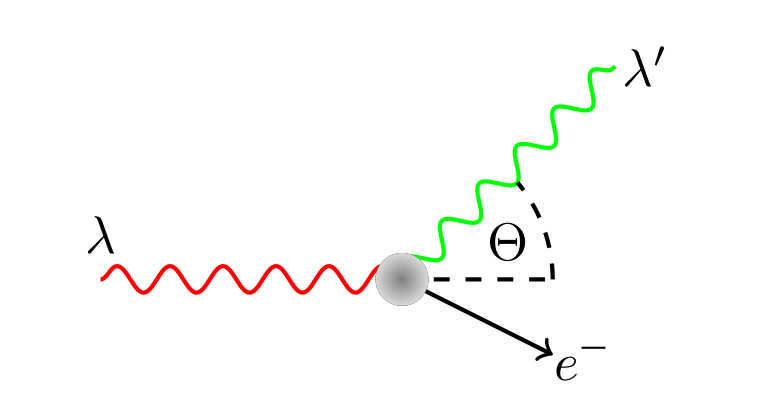
\includegraphics[width=0.3\textwidth]{./fig/photos/scattering.png}
    \label{fig:scattering}
    \caption{An illustration of Compton scattering. The incident photon interacts with the static electron. As the result, new lower energetic photon is emmited in direction changed by $\Theta$ as part of its energy is transferred to electron $e^{-}$. Source: \cite{baca2021gamma}}
\end{figure}

\subsection{Compton camera}
This effect is the fundamental principle in a sensor called a Compton camera. 
The sensor is typically composed of two main components: the scatterer and the absorber. 
The incident photon first interacts with the scatterer, where the lower energetic photon is emitted under angle $\Theta$ (thanks to the Compton effect). 
Since it is more common to measure energies instead of wavelength, we can rewrite the Compton formula as
\begin{equation}
E_{\lambda^{\prime}} = \frac{E_{\lambda}}{  1 + (E_{\lambda} / m_{e}c^{2}) (1 - \mathrm{cos} \Theta)},
\end{equation}
where $E_{\lambda}$ is the energy of the incoming photon from the source, $E_{\lambda^{\prime}}$ is the energy of the scattered photon.  
The bi-product of the interaction (electron $e_{e^{-}}$) is immediately measured in the scatterer, and its position is recorded.
Then, the scattered lower energic photon interacts with the second layer of the sensor - the absorber. 
The photoelectric effect is witnessed while measuring the product of it - the energy of the electron $e_{\lambda^{prime}}$ and its position on the absorber.

Now we can express the scattering angle $\Theta$ as
\begin{equation}
    \Theta = \mathrm{arccos} \left (  1-\frac{m_{e}c^{2}E_{\lambda^{\prime}}}{E_{\lambda} (E_{\lambda} - E_{\lambda^{\prime}})} \right )
    \label{eq:theta}
\end{equation}

Given the measurements on the scatterer and absorber and computed scattering angle $\Theta$ using the equation \ref{eq:theta} (using known energy of the incoming photon $E_{\lambda}$), we can reconstruct a set of possible directions from where the original photon arrived. Since the Compton effect is symmetrical, the set of possible directions towards the source of ionizing radiation forms a surface of a cone.

\subsection{MiniPIX TPX3 sensor}
The sensor used in this work is a small CdTe event-based camera that is capable of witnessing the interactions between gamma photons and the matter of the sensor and reporting them in real time.
Unlike the traditional model of the Compton camera mentioned before, this is a single-stack detector.
In other words, there is no distinction between the scatterer and the absorber and all the measurable interactions are happening in one 14x14x2 mm block of CdTe semiconductor material.
The sensor is capable of measuring a 3D position of the interactions (and distinguishing its type) inside the detector with nanosecond resolution. 
All these features open the possibility of using it in Compton camera mode.
Technical details of the sensor are described in \cite{baca2021gamma} and \cite{baca2019timepix}.
The biggest advantage of this sensor is its small size, low weight and low power consumption.
Thanks to that, we can use this sensor on board a small UAV. 

\begin{figure}[!h]
    \centering
    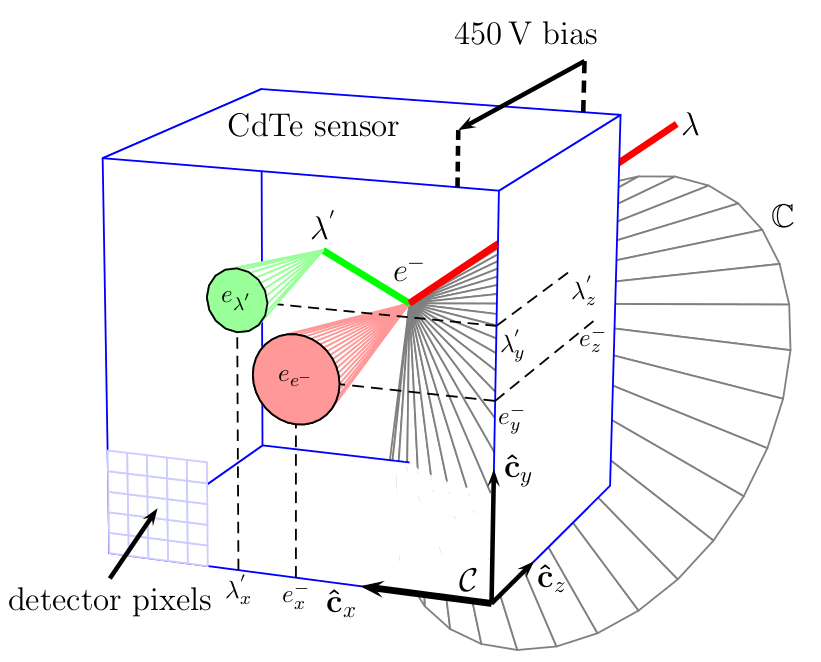
\includegraphics[width=0.3\textwidth]{./fig/photos/minipix.png}
    \label{fig:minipix}
    \caption{An illustration of detection process inside the MiniPIX TPX3 sensor. Source: \cite{baca2021gamma}}
\end{figure}

\section{Localisation of sources of ionizing radiation}

Localisation of sources of ionizing radiation is a well explored and described task in the field of radiotherapy.
One of the frequently used methods is called \ac{MLEM}.
This method is based on widely known EM algorithm (source), which was adapted for radiotherapy (source) and for Compton imagining.
It is an iterative algorithm that tries to estimate number of emmited photons from each cell in the discretised space of all possible source positions.





There are multiple differences between the domain of medical imagining and mapping of radioactive sources using \ac{UAV}s.
The distance between source and detector in radiotherapy is small (tens of centimeters) and number of reconstructed Compton cones is high (tens of thousands).
Other the other hand, distances in robotic exploration scenario are much bigger (meters). 
As we know from the previous section, the intensity of the radiation decreases with the inverse square law.
It means that the source must be reconstructed using much smaller number of compton cones.
Another difference is that \ac{MLEM} is typically used as offline method.
In medical imagining, matrix $\mathbb{T}$ is 




Patients are given some small amount of radioactive material.
The emitted particles are detected using medical sensors based on Compton camera principle.

The input of the method are the Compton cones measured by the drones (each consisting of the origin of the cone, direction of its axis and scattering angle). 

\subsection{Maximum Likelihood Expectation Maximization}

\subsubsection{Maximum likelihood}
Maximum likelihood is a classical approach in machine learning.
In general, it is used for estimating hidden parameters of some hidden underlying probability distribution.
Likelihood can be defined as 
\begin{equation}
  \mathrm{likelihood} = p(\ \mathrm{observations } \  \boldsymbol{O} | \ \mathrm{hidden \ parameters\ } \Phi ).
  \label{eq:likelihood}
\end{equation}
We want to maximise this expression with respect to the hidden parameters.
In other words, we want to find such parameters so that they fit our observations in the best possible way.
%Maximum likelihood is often written with arguments in reversed order as $L(\Phi | \boldsymbol{O} )$, since we want to estimate hidden parameters $\Phi$ using known observations $\boldsymbol{O}$.



\subsubsection{Maximum likelihood Expectation Maximization}

Now lets define the task more formally and derive the algorithm in the general form as presented here \cite{}.
Lets divide the area of possible sources of radiation into $J$ discrete bins (indexed with $j$, where $j = 1 \dotsc J$).
Our observations are divided into $I$ discrete bins and stored in vector $\mathbf{Y}$ (where $y_{i}$ is the number of photons detected in the bin $i$, $i = 1 \dotsc I$).
Then we define a matrix $\mathbf{T}$ ($\mathbf{T} \in \mathbb{R}^{I \times J}$), where each position in the matrix is defined as

\begin{equation}
  t_{ij} =  P(\textrm{detected in } i | \textrm{emitted from } j).
\end{equation}

In other words, $t_{ij}$ represents a probability that we observe observation $i$ given the fact that the radioactive particle was emitted from position $j$.

Lets assume that number of photons emitted from one position $j$ in some time interval is a discrete random variable that follows Poisson distribution with expected value $\lambda_{j}$.
We can fix the time interval to some unit value or to the time duration of the experiment.
Our goal is to estimate $\mathbf{\Lambda}$, which has elements $\lambda_{j}$, each corresponding with expected number of photons emitted from the position $j$.

The likelihood of measuring $y_{i}$ particles in the measurement bin $i$ w.r.t. $\mathbf{\Lambda}$ can be expressed as (Poisson distribution):
\begin{equation}
  p(y_{i} |\mu_{i} ) = e^{-\mu_{i}} \frac{\mu_{i}^{y_i}}{y_{i}!},
\end{equation}
where $\mu_{i} = \sum_{j} t_{ij}\lambda_{j}$ for simplicity denotes the average number of events measured in bin $i$.

The likelihood of all the measurements is
\begin{equation}  
  p(\mathbf{Y} | \mathbf{T\Lambda} ) = \prod_{i} e^{-\mu_{i}} \frac{\mu_{i}^{y_i}}{y_{i}!}.
\end{equation}

After taking its logarithm we have:

\begin{equation}  
  \mathrm{log}\ p(\mathbf{Y} | \mathbf{T\Lambda} ) = \sum_{i}\left ( -\sum_{j} t_{ij}\lambda_{j} + y_{i} \mathrm{log}(\sum_{j} t_{ij}\lambda_{j})  - \mathrm{log}(y_{i}!) \right ).
  \label{eq:likelihood1}
\end{equation}
However, equation \ref{eq:likelihood1} doesn't give an answer to our question - how to determine $\mathbf{\Lambda}$. The solution is to use iterative EM algorithm.

\subsection{Expectation maximization}
The EM algorithm for estimation of log likelihood from incomplete data was proposed in 1977 by \cite{EM}.
It iteratively improves the estimate of parameter we want to optimise ($\Lambda$ in our case).
The values of $\Lambda$ are initialised with some nonzero value.
The EM algorithm typically consists of two stages - \textbf{E step} and \textbf{M step}.

To use the EM algorithm, we need to define the likelihood in a slightly different way.
For that purpose, lets assume that we have (in practice unobservable) complete data $\mathbf{X}$, where $x_{ij}$ represents the fact that the photon emitted from $j$ is detected in $i$ (and all the photons can be detected).
Than we have $E(x_{if}) = t_{ij}\lambda_{j}$ and $y_{i} = \sum_{j}x_{ij}$. 
We can rewrite the log likelihood for complete data as:
\begin{equation}  
  \mathrm{log}\ p(\mathbf{X} | \mathbf{T\Lambda} ) = \sum_{i}\left ( -\sum_{j} t_{ij}\lambda_{j} + x_{i} \mathrm{log}(\sum_{j} t_{ij}\lambda_{j})  - \mathrm{log}(x_{i}!) \right ).
  \label{eq:likelihood2}
\end{equation}

In the \textbf{E step}, we fix the current estimate of $\Lambda$. 
We want to compute the conditional expectation of the log-likelihood with respect to the measured data (with fixed $\Lambda$).



First, we perform the \textbf{E step}.
We fix the current values 
In the \textbf{E step}, we fix the current values of parameters we are trying to estimate.
Than we compute the conditional expectation of the log-likelihood with respect to the measured data.
Then in the \textbf{M step}, we want to find maximum of 


\subsubsection{Poisson distribution}
Poisson distribution is a discrete probability distribution expressing the probability of a given number of events occurring in a fixed interval of time.
We assume that all events are independent of the time since the last event occured.
It can be expressed as:
\begin{equation}
  f(k;\lambda )={\frac {\lambda ^{k}e^{-\lambda }}{k!}},
\end{equation}
where $k$ is the number of events in some time interval and $\lambda$ is an expected value of the distribution.



Our goal is to estimate 

The proposed approach is inspired by a method frequently used in radiotherapy. 
It was introduced in \cite{wilderman}




\begin{equation}
\hat{\lambda}_{j}^{(l+1)} = \frac{\hat{\lambda}_{j}^{(l)}}{s_{j}} \sum_{i \in I} \frac{t_{ij}}{\sum_{k} t_{ik} \hat{\lambda}_{k}^{(l)}}
\end{equation}




We model the number of emmited photons from bin $j$ using so called Poisson distribution.
pOisson distribution is a discrete probability distribution expressing the probability of a given number of events occurring in a fixed interval of time.
We assume that all events are independent of the time since the last event occured.
In our case, the event is a radioactive decay = emmision of a radiactive particle.

In a mathematical notation, we can model it as:
\begin{equation}
  x = 0
\end{equation}


The mapped area is sampled into small bins, indexed as 
\begin{equation}
  m_{j} = 1 ... J
\end{equation}

